\section{Sviluppo di un simulatore di carico cognitivo}
Come si evince da quanto detto fin ora, \emph{il sistema Dashboard per funzionare necessita di interagire con il Database}.\newline

\noindent I dati recuperati dal Database però vengono scritti dalla piattaforma Atlas che, a sua volta, li ha ricevuti dal sistema per l'Acquisizione di segnali.\newline
Al momento della stesura di questo elaborato però \emph{l'algoritmo MindPulse} (all'interno di Atlas) \emph{risulta ancora in fase di perfezionamento e l'applicativo di Acquisizione in fase di sviluppo}.\newline

\noindent Per verificare dunque il corretto funzionamento della Dashboard, è nata l'idea di sviluppare un {\bf simulatore di carico cognitivo} \emph{che vada a sostituirsi alla piattaforma Atlas nella scrittura di dati sul database MongoDB}.
\subsection{Ruolo del simulatore nel sistema NeuroFrame}
Il simulatore rende possibile ottenere continuamente nuovi dati sul Database così che la Dashboard possa mostrarli seguendo il suo normale funzionamento.\newline
La \emph{figura 5.1} riprende quanto visto precedentemente nella \emph{figura 3.1}, escludendo però Atlas ed App di acquisizione e sostituendoli con il simulatore.
\vspace{5mm}
\begin{figure}[H]
  \centering
  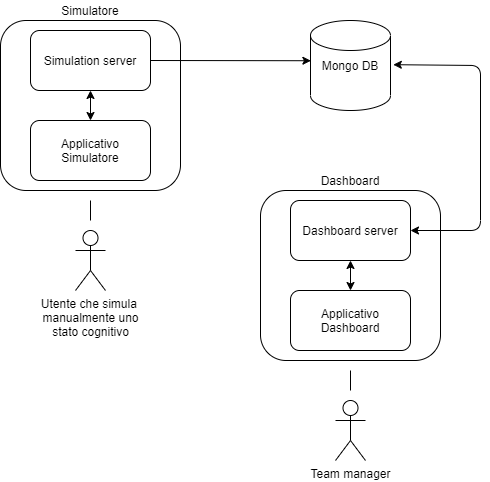
\includegraphics[width=0.7\textwidth]{img/NeuroFrameSimulatore.png}
  \caption{Architettura di NeuroFrame con simulatore di carico cognitivo}
\end{figure}
\vspace{5mm}
\noindent Data la volontà di Vibre di creare altri progetti (che sfruttano gli algoritmi della piattaforma) la cui architettura segua un'impostazione molto similare a NeuroFrame, \emph{il simulatore è stato pensato con l'idea di essere riutilizzabile in altri contesti}.\newline

\noindent Per correttezza infatti, \emph{l'applicativo andrebbe visto come uno scrittore di dati su database a cadenza periodica}, piuttosto che come un simulatore prettamente legato a NeuroFrame; 
Il progetto prende dunque il nome di {\bf Simulatore di Piattaforma}, simulando l'output su database di quest'ultima.

\noindent Se normalmente la Piattaforma Atlas elaborerebbe un input biometrico al fine di fornire metriche da utilizzare, \emph{l'utente del Simulatore invece manipola manualmente il valore di tali metriche da inviare al database}, simulando il variare dei risultati ottenuti dagli algoritmi della piattaforma.\newline

\noindent Al fine di rendere il Simulatore utilizzabile in più progetti, \emph{l'utente potrà creare delle configurazioni che specifichino quali dati inviare, in che collezioni e in quale database}.
\subsection{Flusso d' informazione in relazione agli altri componenti}
Vediamo ora come il simulatore comunica con le componenti di NeuroFrame.\newline
Il flusso d'informazione lato Dashboard, essendo esso un sottosistema che comunica principalmente con il Database, rimane invariato rispetto a quanto descritto nella \emph{sezione 3.3}.\newline

\noindent Il Simulatore invece va a sostituire il flusso informativo lato Applicativo di acquisizione, con una comunicazione più breve dovuta al fatto che sono coinvolti meno sistemi ed i dati non vengono elaborati dall'algoritmo MindPulse, ma direttamente decisi dall'utente che utilizza il Simulatore.\newline
La logica alla base della comunicazione rimane invariata, inviando dati a MongoDB secondo una cadenza periodica.
\vspace{10mm}
\begin{figure}[H]
  \centering
  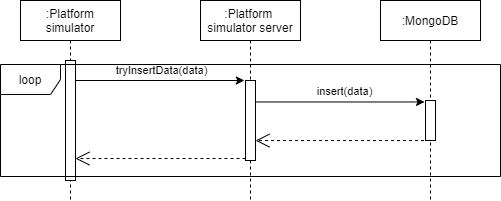
\includegraphics[width=1.0\textwidth]{img/diagramma_sequenza_simulatore.png}
  \caption{Diagramma di sequenza rappresentante il flusso informativo dal Simulatore a MongoDB}
\end{figure}

\subsection{Soluzioni tecnologiche utilizzate}
Analogamente al sistema Dashboard, il Simulatore è composto da due applicativi:
\begin{itemize}
  \item \emph{Un server realizzato tramite Node.js, con il supporto del framework Express (vedi sezione 4.2.2)}
  \item \emph{L'applicativo con cui l'utente interagisce, sviluppato anch'esso tramite Node.js con l'ausilio del framework React (vedi sezione 4.1.1)}
\end{itemize}
Differentemente dall'applicativo Dashboard \emph{non è stato necessario l'utilizzo di Redux} (\emph{sezione 4.1.2}) in quanto l'applicativo risulta di essere di dimensioni molto contenute, rendendo gli strumenti offerti da React più che sufficienti per lo scopo.\newline

\noindent Al fine di salvare delle configurazioni da riutilizzare in futuro, è stato implementato un \emph{salvataggio di file locali} contenenti tutti i parametri necessari al fine di ripristinare tale configurazione; tali file contengono una \emph{struttura in formato JSON} con il setting creato dall'utente. 